\documentclass{article}

%% Downloading Packages for the Document.

\usepackage{datetime} % Dates.
\usepackage{fancyhdr} % Headers.
\usepackage{lastpage} % Page References.

\usepackage{graphicx} % Inserting Images.
\usepackage{float} % Postitioning Images.

\usepackage{dirtytalk} % Speech & Quote Marks.
\usepackage{hyperref} % Hyperlinks and References.
\usepackage{xcolor} % Coloured Text.
\usepackage{enumitem} % Letter Bullets. 
% \begin{enumerate}[label=\alph*.] 

\usepackage{amssymb} % Maths Symbols.
\usepackage{amsmath} % Maths Tools.

\usepackage{algpseudocode} % Pseudocode.
\usepackage{algorithm} % Algorithms.

\usepackage[margin=1in]{geometry} % Margins.

%%


%% Creating Formats.

\hypersetup{colorlinks=true, urlcolor=blue, linkcolor=black}

\newdateformat{monthyeardate}
{%
    \monthname[\THEMONTH] \THEYEAR
}

\newdateformat{yeardate}
{%
    \THEYEAR
}

% Colouring and Spacing.
\newcommand{\colour}[2] {\color{#1}#2\color{black}}
\newcommand{\separate}[1] {\vspace{#1 pt}\noindent}

% Maths Number Sets.
\newcommand{\R}{\mathbb{R}}
\newcommand{\N}{\mathbb{N}}
\newcommand{\C}{\mathbb{C}}
\newcommand{\Q}{\mathbb{Q}}
\newcommand{\Z}{\mathbb{Z}}

% Document Colour Scheme.
\newcommand{\definition}[2]{\textbf{Definition #1}: #2 }
\newcommand{\theorem}[2]{\textbf{Theorem #1}: #2 }
\newcommand{\lemma}[2]{\textbf{Lemma #1}: #2 }

%%


%% Setting up the Document.

\title{Partitions}
\author{MATTHEW EMERSON}
\date{\monthyeardate\today} % Edit this to get a static date.

\begin{document}

%%


%% Setting the Default Header and Footer. 

\pagestyle{fancy}
\fancyfoot{}
\fancyfoot[L]{Written by Matthew Emerson \\ \textit{\LaTeX \,Template: Copyright \date{\yeardate\today}, Matthew Emerson}}
\fancyfoot[R]{Page \thepage \, of\, \pageref{LastPage}}

%%


%% Creating the Title Page.

\maketitle
\thispagestyle{empty}

%% 


%% Creating the Table of Contents Page.

\newpage
\thispagestyle{empty}

\tableofcontents

%% 


%% The Main Document.

\setcounter{page}{0}
\newpage

\section{Introduction to Partitions}

\definition{1.1}{A \underline{partition} of \(n \in \N\) is a way of writing \(n\) as the sum of numbers.} These will be denoted in this document as \((p_1+p_2+...+p_i) \vdash n\).

\separate{5}\definition{1.2}{A \underline{part} is one of the numbers that make up a partition. It has an associated \underline{part size}, which is the value of the number.}

\separate{5}\definition{1.3}{The \underline{partition function} of \(n\) is the number of possible partitions of \(n\).} This will be denoted as \(p(n) = i\).

\separate{5}\definition{1.4}{The \underline{set of partitions} is the set containing all possible partitions of \(n\).} This will be denoted using non-standard notation as \(P(n) = \{p_1, p_2, ..., p_i\}\) where \(p_x\) is a partition of \(n\) and \(i = p(n)\).

\separate{5}\definition{1.5}{\underline{Conditional partitions} can also be created which limit which partitions are valid based on a given condition.} This can be applied to both partition functions and sets of partitions as \(p(n|condition)\) and \(P(n|condition)\).

\section{Bijective Proofs and Euler's Identity}

\subsection{Bijective Proofs}

\definition{2.1.1}{A \underline{bijection} is a mathematical function that is a one-to-one and onto mapping (Merriam-Webster, 2025).} 

\separate{5}We can prove that there is a bijection between two sets \(A\) and \(B\) by defining the functions \(f:A \rightarrow B\) and \(f^{-1}: B \rightarrow A\). This can be useful when trying to compare the size of two partition functions that would be hard to compute as if there is a bijection between two sets of partitions, the corresponding partition functions will be equal.

\separate{5}\textbf{Proof 2.1.1}\label{proof:2.1.1}: We can prove that, for any \(n \geq 1, n \in \N,\)\
\[p(n | \textit{all parts are even}) = p(n | \textit{even number of parts})\]
To prove that these partition functions are equal using a bijection, let \(A = P(n| \textit{all parts are even})\) and \(B = P(n | \textit{even number of parts})\).

We can then define $f:A \rightarrow B$ to be the following: For each partition $a \in A$, take its corresponding parts, and replace each of them with two parts half the size. The resulting partition should be a member of $B$.
\[f: (2a_1 + 2a_2 + ... + 2a_n) \rightarrow (a_1 + a_1 + a_2 + a_2 + ... + a_n + a_n)\]
Similarly, we can define $f^{-1}: B \rightarrow A$ as: For each partition $b \in B$, we take its parts and pair each of them with one of corresponding value. These pairs are then replaced with a single part, double the size of the original. The resulting partition should be a member of $A$.
\[f^{-1}: ((a_1 + a_1) + (a_2 + a_2) + ... + (a_n + a_n)) \rightarrow (2a_1 + 2a_2 + ... + 2a_n)\]
If we take a partition from \(A\), apply \(f\), then apply \(f^{-1}\), the resulting partition will be the same partition we started with. This means there must be a bijection between \(A\) and \(B\), therefore, for any \(n \geq 1, n \in \N,\)
\[p(n | \textit{all parts are even}) = p(n | \textit{even number of parts})\]

\subsection{Euler's Identity}

\definition{2.2.1}{\underline{Euler's Identity} states that, for any positive integer \(n\),
\[p(n|\textit{each part is odd}) = p(n|\textit{each part is distinct})\]}
This identity can be further generalised to get

\separate{5}\theorem{2.2.1}{For any pair of integers, \(k \geq 2, \; n \geq 1\),
\[p(n|\textit{no part is a multiple of } k) = p(n|\textit{each part is repeated at most } k-1 \,{times})\]}
\textbf{Proof 2.2.1}: Let 
\begin{itemize}
    \item \(A = P(n|\textit{no part is a multiple of } k)\)
    \item \(B = P(n|\textit{each part is repeated at most } k-1 \,{times})\)
\end{itemize}
This again can be proved with a bijection. We define \(f:A\rightarrow B\) to be an iterative function which recursively checks a partition from \(A\) for instances of part sizes which appear at least \(k\) times. The function then takes these \(k\)-length tuples, and replaces them with a new part with size \(k\)-times the original size. Once no part size appears more than \(k-1\) times, the resulting partition will be a member of \(B\).
\[f: ((x_1+x_2+...+x_k)+ y + ...) \rightarrow (kx + y + ...)\]
We can then define \(f^{-1}:B \rightarrow A\) as taking a partition from \(B\) any parts whose size is a multiple of \(k\) and replacing them with a \(k\)-length tuple of parts whose sizes are \(k\)-times smaller. After all part size multiples of \(k\) are replaced, the resulting partition will be a member of \(A\).
\[f^{-1}: (kx + y + ...) \rightarrow ((x_1 + x_2 + ... + x_k) + y + ...)\]
Then, if we took a partition from \(A\), applied \(f\) and \(f^{-1}\), the resulting partition would be identical to the original partition, proving that, for any pair of integers, \(k \geq 2, \; n \geq 1\),
\[p(n|\textit{no part is a multiple of } k) = p(n|\textit{each part is repeated at most } k-1 \,{times})\]

\newpage
\section{Euler Pairs and Alder's Conjecture}

\colour{red}{THIS SECTION HAS NOT BEEN WRITTEN YET - AND FIX THE DIAGRAMS}
\newpage

\section{Young Diagrams and Ferrers Graphs}

\definition{4.1}{\underline{Young diagrams} represent partitions by stacking rows of squares (corresponding to individual parts) on top of each other, in ascending order (See \hyperref[fig:visualisationOptions]{Figure 1(a)}).}

\separate{5}\definition{4.2}{\underline{Ferrers graphs} represent partitions in a similar way, but instead electing to utilise dots instead of squares when representing parts (See \hyperref[fig:visualisationOptions]{Figure 1(b)}).} 

\begin{figure}[H]
    \centering
    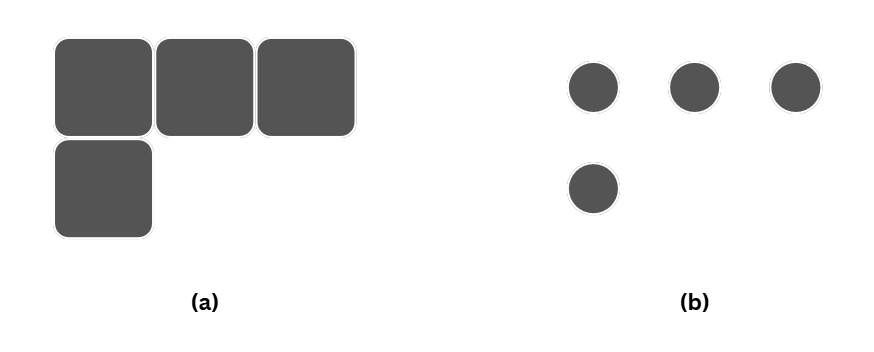
\includegraphics[width=0.4\linewidth]{Images/Visualisation Options.png}
    \caption{Visualisation Options}
    \label{fig:visualisationOptions}
\end{figure}

\noindent From this point, I will be using Ferrers diagrams as my preferred choice of visualisation, but Young diagrams would be equally valid.

\subsection{Solving Problems with Visualisations}

\textbf{Proof 4.1.1}: Previously, in \hyperref[proof:2.1.1]{Example 2.1.1}, we used a bijection to prove that, for any \(n \geq 1, n \in \N,\)
\[p(n | \textit{all parts are even}) = p(n | \textit{even number of parts})\]
This can similarly be achieved using Ferrers graphs by redefining \(f\) and \(f^{-1}\) to be the following:
\begin{itemize}
    \item \(f\) can be defined as taking a partition from \(A\), and splitting each constituent part (row of the diagram) down the middle, and using the results to create two new rows. This resulting partition will be a member of \(B\).
    \item Similarly, we can define \(f^{-1}\) as taking a partition from \(B\), combining parts of equal size into one row, and adding that as a new part. This results in a partition from \(A\).
\end{itemize}
As we can see in \hyperref[fig:problem4.1.1]{Figure 2}, when the functions are applied in turn to an example partition from \(A\), the resulting partition is also a member of \(A\) while the middle partition is in \(B\). This demonstrates the bijection between the sets and again proves that, for any \(n \geq 1, n \in \N,\)
\[p(n | \textit{all parts are even}) = p(n | \textit{even number of parts})\]

\begin{figure}[H]
    \centering
    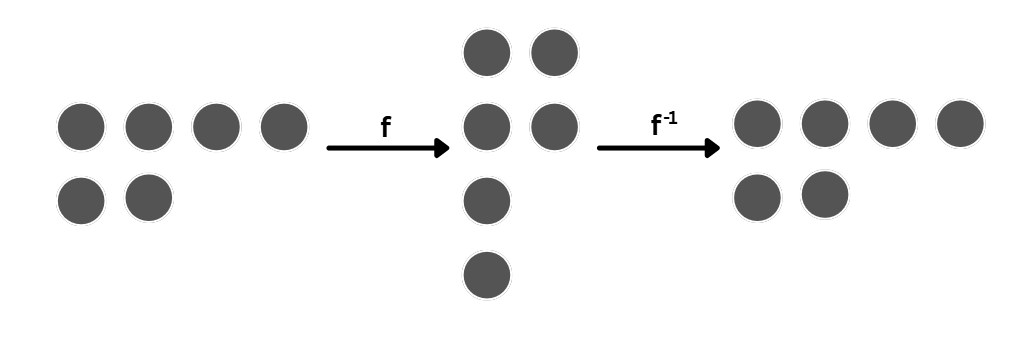
\includegraphics[width=0.5\linewidth]{Images/Problem 4.1.1.png}
    \caption{Applying \(f\) and \(f^{-1}\)}
    \label{fig:problem4.1.1}
\end{figure}

\section{Partition Conjugates}

\definition{5.1}{A \underline{conjugate} of a partition is a partition which has had its rows and columns transposed to give a new partition.}

\separate{5}\definition{5.2}{A \underline{self-conjugate partition} is a partition which is a conjugate of itself; meaning that the original partition is the same as the transposed version.}

\separate{5}This can produce some interesting results, such as proving that, for any \(n \geq 1, n \in \N\), 
\[p(n|\textit{self-conjugate}) = p(n|\textit{all parts are both distinct and odd)}\]
\textbf{Proof 5.1}: This can be again be proved by creating a bijection between the sets \(A = P(n|\textit{self-conjugate})\) and \(B = P(n|\textit{all parts are both distinct and odd})\).

We can define the function \(f:A \rightarrow B\) to be: taking a partition from \(A\), recursively take the dots making up both the first row and column of the Ferrers diagram and form a new row. This is guaranteed to be an odd number as the row and column will be the same length, and will share one dot. This will result in a partition from \(B\).

\(f^{-1}\) can then be defined as: taking a partition from \(B\), take each part, starting from the bottom, get its size \(i\), and create one part of size \(\frac{i}{2}+1\), and \(\frac{i}{2}-1\) parts of size one. This can then be nested inside the previous row. The resulting partition will be a member of \(A\).

When applied in turn on a partition from \(A\), this creates a partition from \(B\) and then returns it back to the original state, demonstrating the bijection, and proving that for any \(n \geq 1, n \in \N\), 
\[p(n|\textit{self-conjugate}) = p(n|\textit{all parts are both distinct and odd)}\]

\begin{figure}[H]
    \centering
    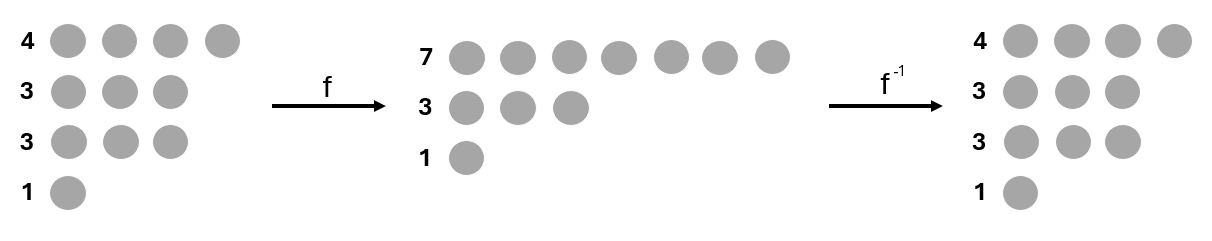
\includegraphics[width=1\linewidth]{Images/Problem 5.1.png}
    \caption{Applying \(f\) and \(f^{-1}\)}
    \label{fig:problem5.1}
\end{figure}

\section{How Big is \textit{p(n)}?}

\colour{red}{HERE ONWARDS HAS NOT BEEN WRITTEN YET}

\section{Durfee Squares}

\newpage\section{Generating Functions}

\newpage\section*{References}
\addcontentsline{toc}{section}{References}

Durham University (2026). \textit{Partitions: Worksheet 1-4}.

\separate{10}Merriam-Webster (2025). \textit{BIJECTION Definition \& Meaning - Merriam Webster}. [online] \\ Merriam-webster.com. Available at: https://www.merriam-webster.com/dictionary/bijection \\ \([\text{Accessed 9 Mar. 2026}]\).

\end{document}

%%